\documentclass{resume}
\usepackage{NotoSerifCJKsc_external}
\usepackage{linespacing_fix}
\usepackage{hyperref}
\usepackage{fontawesome}
\usepackage{graphicx}
\usepackage{booktabs} 

\begin{document}
\pagenumbering{gobble}

\noindent
\begin{minipage}[c][][c]{0.75\textwidth}
    
    \vspace*{0.5cm}

    \begin{tabular}{l@{\hspace{2.2cm}}l}
        \faUser\ 姓名:王健 & \faMapMarker\ 籍贯:江西 宜春 \\
        \addlinespace[3.5mm]
        \faEnvelope\ \href{mailto:jona.wzu@gmail.com}{jona.wzu@gmail.com} & \faBirthdayCake\ 出生年月:1999.04 \\
        \addlinespace[3.5mm]
        \faPhone\ (+86) 157-7054-6370 & \faGithub\ \href{https://github.com/aajonaa}{https://github.com/aajonaa} \\ 
    \end{tabular}
    
    \vspace*{0.5cm}

\end{minipage}
\hspace{0.05\textwidth}
\begin{minipage}[c][][c]{0.2\textwidth}
    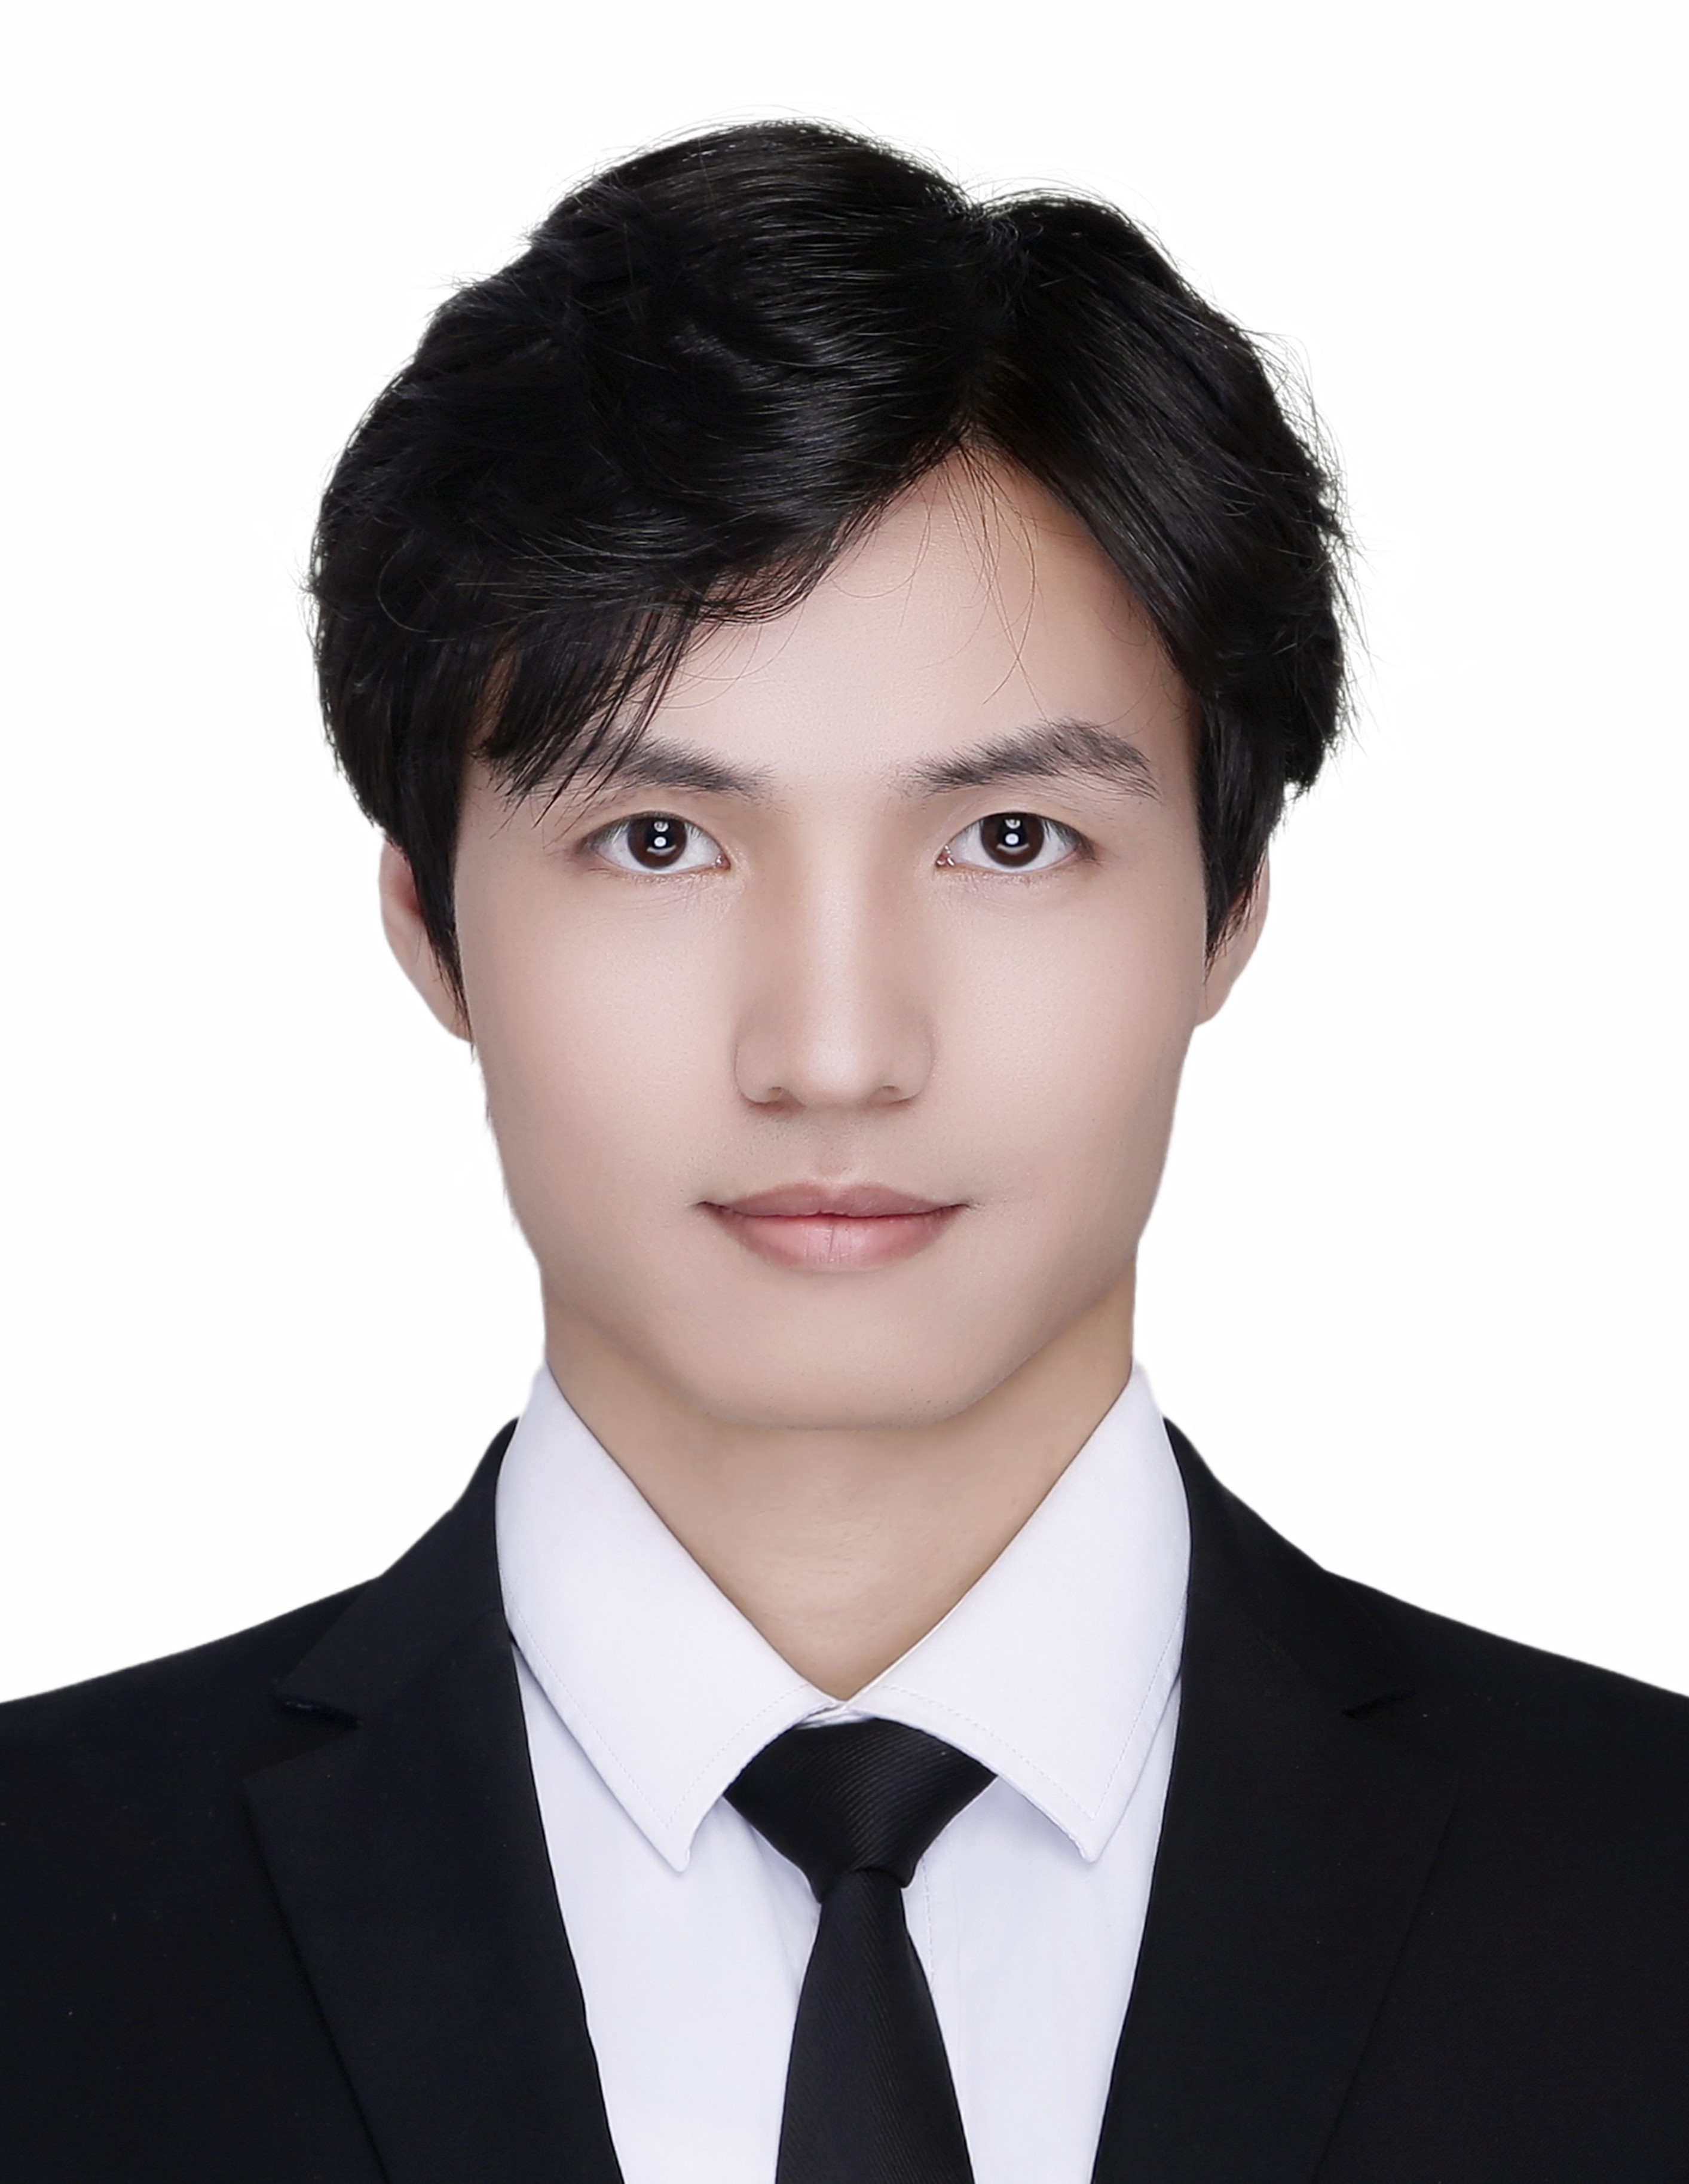
\includegraphics[width=\linewidth]{profile_2_mod.jpg} 
\end{minipage}

\vspace{0.4cm}

\section{\faGraduationCap\ 教育背景}
\datedsubsection{\textbf{温州大学}, 温州}{2023 -- 至今}
\textit{硕士研究生在读} \quad 计算机科学与技术 \quad 预计2026年6月毕业\\
导师:陈慧灵教授 课题组:医学数据挖掘与计算智能实验室

\begin{itemize}
  \item 2023年新生学业二等奖学金
  \item 2023-2024学年温州大学一等奖学金
  \item 计算机之光校友基金英才奖
\end{itemize}

\datedsubsection{\textbf{江西理工大学}, 南昌}{2018 -- 2022}
\textit{工学学士} \quad 软件工程

\section{\faFileTextO\ 学术成果}
\begin{itemize}
  \item \textbf{Wang J}, Chen Y, Lu C, Heidari A A, Wu Z, Chen H.\\
  \textbf{The Status-based Optimization: Algorithm and comprehensive performance analysis}.\\
  \textit{Neurocomputing}, 2025. (SCI二区, CCF-C, IF=6.5)

  \item \textbf{Wang J}, Chen Y, Lu C, Heidari A A, Liu L, Chen H.\\
  \textbf{Bandit-Driven Adaptive Search in Surrogate-Assisted Evolutionary Algorithm with Explainable Uncertainty Criteria}.\\
  \textit{Swarm and Evolutionary Computation}, 2025. (SCI二区, IF=8.5, 一修中)
\end{itemize}

\section{\faKey\ 知识产权}
\begin{itemize}
  \item \textbf{发明专利}(第2发明人):一种多阈值图像分割方法、装置、计算机设备及存储介质\\
  申请号:2025110129939(受理中)
  \item \textbf{软件著作权}(3/5):基于深度学习模型的肺炎辅助诊断系统 V1.0\\
  登记号:2024SR1062875
\end{itemize}

\section{\faTrophy\ 获奖情况}
\begin{itemize}
  \item \textbf{银奖}(1/15),“建行杯”浙江省国际大学生创新大赛(2024)
  \item \textbf{铜奖}(3/15),第十四届“挑战杯”秦创原中国大学生创业计划竞赛“一带一路”国际邀请赛全国总决赛
  \item \textbf{银奖}(1/15),2024年“新湖杯”温州大学大学生创新大赛
  \item \textbf{金奖}(4/15),温州大学第十一届“挑战杯”大学生课外学术科技作品竞赛决赛(2024)
  \item \textbf{优胜奖}(2/5),2024年“共创未来”中美青年创客大赛温州分赛区
  \item \textbf{优秀奖}(1/5),2024年“数据要素X”大赛浙江分赛温州站
\end{itemize}

\section{\faUsers\ 项目经历}
\datedsubsection{\textbf{构建肺部疾病早筛辅助系统}}{2025年}
\role{项目成员(共5人,排名第3)}{大学生科技创新活动(暨新苗人才计划)项目,指导老师:陈慧灵、陈翼、李成业}
\begin{itemize}
  \item 与宋昊杲、郑博利、王炜炜、赵苑利合作,联合开发肺部CT图像智能分析系统,实现早期病变辅助诊断
\end{itemize}

\section{\faCogs\ 技术能力}
\begin{itemize}[parsep=0.5ex]
  \item \textbf{编程语言}: Python > C > C++ > Matlab
  \item \textbf{开发平台}: Linux,Visual Studio Code,Git
  \item \textbf{工具与框架}: PyTorch, LaTeX
\end{itemize}

\section{\faHeartO\ 其他信息}
\begin{itemize}[parsep=0.5ex]
  \item 英语能力: 英语六级(CET6),听说读写熟练
\end{itemize}

\end{document}